% Created by tikzDevice version 0.12
% !TEX encoding = UTF-8 Unicode
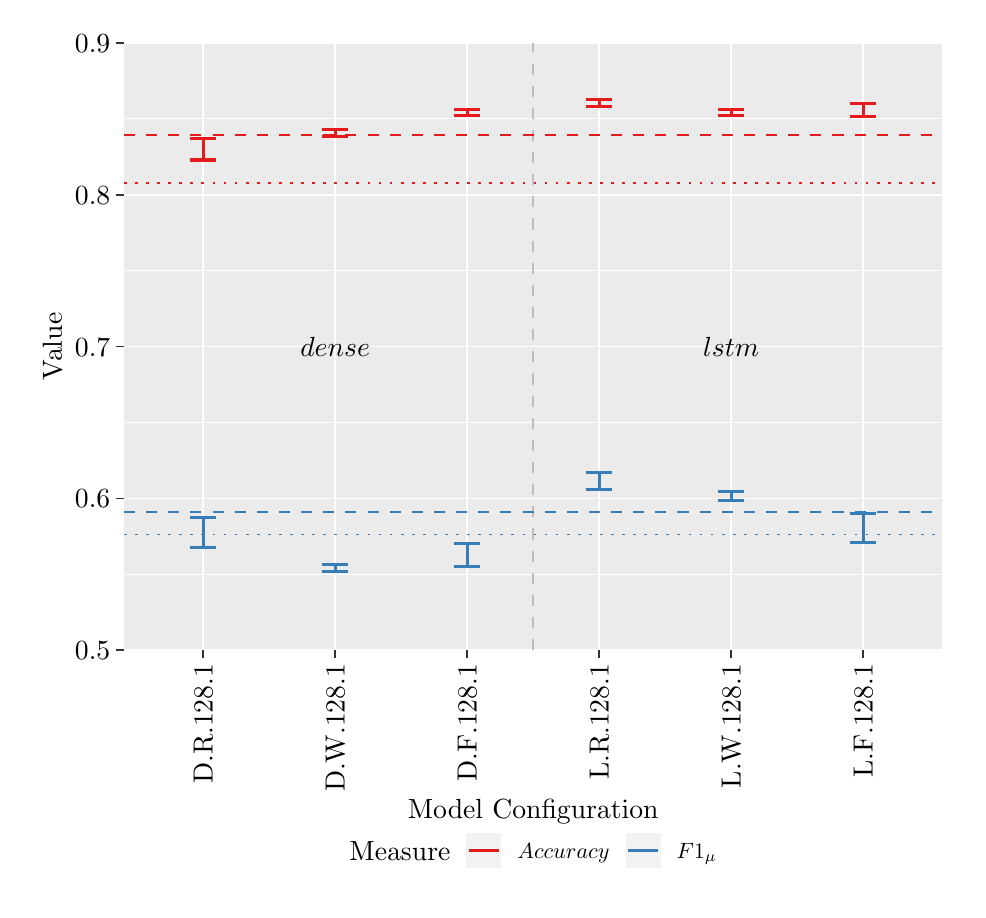
\begin{tikzpicture}[x=1pt,y=1pt]
\definecolor{fillColor}{RGB}{255,255,255}
\path[use as bounding box,fill=fillColor,fill opacity=0.00] (0,0) rectangle (336.00,311.47);
\begin{scope}
\path[clip] (  0.00,  0.00) rectangle (336.00,311.47);
\definecolor{drawColor}{RGB}{255,255,255}
\definecolor{fillColor}{RGB}{255,255,255}

\path[draw=drawColor,line width= 0.6pt,line join=round,line cap=round,fill=fillColor] (  0.00,  0.00) rectangle (336.00,311.47);
\end{scope}
\begin{scope}
\path[clip] ( 34.81, 86.52) rectangle (330.50,305.97);
\definecolor{fillColor}{gray}{0.92}

\path[fill=fillColor] ( 34.81, 86.52) rectangle (330.50,305.97);
\definecolor{drawColor}{RGB}{255,255,255}

\path[draw=drawColor,line width= 0.3pt,line join=round] ( 34.81,113.95) --
	(330.50,113.95);

\path[draw=drawColor,line width= 0.3pt,line join=round] ( 34.81,168.81) --
	(330.50,168.81);

\path[draw=drawColor,line width= 0.3pt,line join=round] ( 34.81,223.68) --
	(330.50,223.68);

\path[draw=drawColor,line width= 0.3pt,line join=round] ( 34.81,278.54) --
	(330.50,278.54);

\path[draw=drawColor,line width= 0.6pt,line join=round] ( 34.81, 86.52) --
	(330.50, 86.52);

\path[draw=drawColor,line width= 0.6pt,line join=round] ( 34.81,141.38) --
	(330.50,141.38);

\path[draw=drawColor,line width= 0.6pt,line join=round] ( 34.81,196.25) --
	(330.50,196.25);

\path[draw=drawColor,line width= 0.6pt,line join=round] ( 34.81,251.11) --
	(330.50,251.11);

\path[draw=drawColor,line width= 0.6pt,line join=round] ( 34.81,305.97) --
	(330.50,305.97);

\path[draw=drawColor,line width= 0.6pt,line join=round] ( 63.42, 86.52) --
	( 63.42,305.97);

\path[draw=drawColor,line width= 0.6pt,line join=round] (111.11, 86.52) --
	(111.11,305.97);

\path[draw=drawColor,line width= 0.6pt,line join=round] (158.81, 86.52) --
	(158.81,305.97);

\path[draw=drawColor,line width= 0.6pt,line join=round] (206.50, 86.52) --
	(206.50,305.97);

\path[draw=drawColor,line width= 0.6pt,line join=round] (254.19, 86.52) --
	(254.19,305.97);

\path[draw=drawColor,line width= 0.6pt,line join=round] (301.88, 86.52) --
	(301.88,305.97);
\definecolor{drawColor}{RGB}{190,190,190}

\path[draw=drawColor,line width= 0.6pt,dash pattern=on 4pt off 4pt ,line join=round] (182.65, 86.52) -- (182.65,305.97);
\definecolor{drawColor}{RGB}{0,0,0}

\node[text=drawColor,anchor=base,inner sep=0pt, outer sep=0pt, scale=  1.00] at (111.11,192.79) {\(dense\)};

\node[text=drawColor,anchor=base,inner sep=0pt, outer sep=0pt, scale=  1.00] at (254.19,192.79) {\(lstm\)};
\definecolor{drawColor}{RGB}{228,26,28}

\path[draw=drawColor,line width= 0.6pt,dash pattern=on 4pt off 4pt ,line join=round] ( 34.81,272.78) -- (330.50,272.78);

\path[draw=drawColor,line width= 0.6pt,dash pattern=on 1pt off 3pt ,line join=round] ( 34.81,255.30) -- (330.50,255.30);
\definecolor{drawColor}{RGB}{55,126,184}

\path[draw=drawColor,line width= 0.6pt,dash pattern=on 4pt off 4pt ,line join=round] ( 34.81,136.38) -- (330.50,136.38);

\path[draw=drawColor,line width= 0.6pt,dash pattern=on 1pt off 3pt ,line join=round] ( 34.81,128.28) -- (330.50,128.28);
\definecolor{drawColor}{RGB}{228,26,28}

\path[draw=drawColor,line width= 1.1pt,line join=round] ( 58.65,271.58) --
	( 68.19,271.58);

\path[draw=drawColor,line width= 1.1pt,line join=round] ( 63.42,271.58) --
	( 63.42,263.65);

\path[draw=drawColor,line width= 1.1pt,line join=round] ( 58.65,263.65) --
	( 68.19,263.65);

\path[draw=drawColor,line width= 1.1pt,line join=round] ( 58.65,271.58) --
	( 68.19,271.58);

\path[draw=drawColor,line width= 1.1pt,line join=round] ( 63.42,271.58) --
	( 63.42,263.65);

\path[draw=drawColor,line width= 1.1pt,line join=round] ( 58.65,263.65) --
	( 68.19,263.65);

\path[draw=drawColor,line width= 1.1pt,line join=round] ( 58.65,271.58) --
	( 68.19,271.58);

\path[draw=drawColor,line width= 1.1pt,line join=round] ( 63.42,271.58) --
	( 63.42,263.65);

\path[draw=drawColor,line width= 1.1pt,line join=round] ( 58.65,263.65) --
	( 68.19,263.65);

\path[draw=drawColor,line width= 1.1pt,line join=round] ( 58.65,271.58) --
	( 68.19,271.58);

\path[draw=drawColor,line width= 1.1pt,line join=round] ( 63.42,271.58) --
	( 63.42,263.65);

\path[draw=drawColor,line width= 1.1pt,line join=round] ( 58.65,263.65) --
	( 68.19,263.65);

\path[draw=drawColor,line width= 1.1pt,line join=round] ( 58.65,271.58) --
	( 68.19,271.58);

\path[draw=drawColor,line width= 1.1pt,line join=round] ( 63.42,271.58) --
	( 63.42,263.65);

\path[draw=drawColor,line width= 1.1pt,line join=round] ( 58.65,263.65) --
	( 68.19,263.65);

\path[draw=drawColor,line width= 1.1pt,line join=round] ( 58.65,271.58) --
	( 68.19,271.58);

\path[draw=drawColor,line width= 1.1pt,line join=round] ( 63.42,271.58) --
	( 63.42,263.65);

\path[draw=drawColor,line width= 1.1pt,line join=round] ( 58.65,263.65) --
	( 68.19,263.65);

\path[draw=drawColor,line width= 1.1pt,line join=round] ( 58.65,271.58) --
	( 68.19,271.58);

\path[draw=drawColor,line width= 1.1pt,line join=round] ( 63.42,271.58) --
	( 63.42,263.65);

\path[draw=drawColor,line width= 1.1pt,line join=round] ( 58.65,263.65) --
	( 68.19,263.65);

\path[draw=drawColor,line width= 1.1pt,line join=round] ( 58.65,271.58) --
	( 68.19,271.58);

\path[draw=drawColor,line width= 1.1pt,line join=round] ( 63.42,271.58) --
	( 63.42,263.65);

\path[draw=drawColor,line width= 1.1pt,line join=round] ( 58.65,263.65) --
	( 68.19,263.65);

\path[draw=drawColor,line width= 1.1pt,line join=round] (106.34,274.67) --
	(115.88,274.67);

\path[draw=drawColor,line width= 1.1pt,line join=round] (111.11,274.67) --
	(111.11,272.08);

\path[draw=drawColor,line width= 1.1pt,line join=round] (106.34,272.08) --
	(115.88,272.08);

\path[draw=drawColor,line width= 1.1pt,line join=round] (106.34,274.67) --
	(115.88,274.67);

\path[draw=drawColor,line width= 1.1pt,line join=round] (111.11,274.67) --
	(111.11,272.08);

\path[draw=drawColor,line width= 1.1pt,line join=round] (106.34,272.08) --
	(115.88,272.08);

\path[draw=drawColor,line width= 1.1pt,line join=round] (106.34,274.67) --
	(115.88,274.67);

\path[draw=drawColor,line width= 1.1pt,line join=round] (111.11,274.67) --
	(111.11,272.08);

\path[draw=drawColor,line width= 1.1pt,line join=round] (106.34,272.08) --
	(115.88,272.08);

\path[draw=drawColor,line width= 1.1pt,line join=round] (106.34,274.67) --
	(115.88,274.67);

\path[draw=drawColor,line width= 1.1pt,line join=round] (111.11,274.67) --
	(111.11,272.08);

\path[draw=drawColor,line width= 1.1pt,line join=round] (106.34,272.08) --
	(115.88,272.08);

\path[draw=drawColor,line width= 1.1pt,line join=round] (106.34,274.67) --
	(115.88,274.67);

\path[draw=drawColor,line width= 1.1pt,line join=round] (111.11,274.67) --
	(111.11,272.08);

\path[draw=drawColor,line width= 1.1pt,line join=round] (106.34,272.08) --
	(115.88,272.08);

\path[draw=drawColor,line width= 1.1pt,line join=round] (106.34,274.67) --
	(115.88,274.67);

\path[draw=drawColor,line width= 1.1pt,line join=round] (111.11,274.67) --
	(111.11,272.08);

\path[draw=drawColor,line width= 1.1pt,line join=round] (106.34,272.08) --
	(115.88,272.08);

\path[draw=drawColor,line width= 1.1pt,line join=round] (106.34,274.67) --
	(115.88,274.67);

\path[draw=drawColor,line width= 1.1pt,line join=round] (111.11,274.67) --
	(111.11,272.08);

\path[draw=drawColor,line width= 1.1pt,line join=round] (106.34,272.08) --
	(115.88,272.08);

\path[draw=drawColor,line width= 1.1pt,line join=round] (106.34,274.67) --
	(115.88,274.67);

\path[draw=drawColor,line width= 1.1pt,line join=round] (111.11,274.67) --
	(111.11,272.08);

\path[draw=drawColor,line width= 1.1pt,line join=round] (106.34,272.08) --
	(115.88,272.08);

\path[draw=drawColor,line width= 1.1pt,line join=round] (154.04,281.81) --
	(163.58,281.81);

\path[draw=drawColor,line width= 1.1pt,line join=round] (158.81,281.81) --
	(158.81,279.73);

\path[draw=drawColor,line width= 1.1pt,line join=round] (154.04,279.73) --
	(163.58,279.73);

\path[draw=drawColor,line width= 1.1pt,line join=round] (154.04,281.81) --
	(163.58,281.81);

\path[draw=drawColor,line width= 1.1pt,line join=round] (158.81,281.81) --
	(158.81,279.73);

\path[draw=drawColor,line width= 1.1pt,line join=round] (154.04,279.73) --
	(163.58,279.73);

\path[draw=drawColor,line width= 1.1pt,line join=round] (154.04,281.81) --
	(163.58,281.81);

\path[draw=drawColor,line width= 1.1pt,line join=round] (158.81,281.81) --
	(158.81,279.73);

\path[draw=drawColor,line width= 1.1pt,line join=round] (154.04,279.73) --
	(163.58,279.73);

\path[draw=drawColor,line width= 1.1pt,line join=round] (154.04,281.81) --
	(163.58,281.81);

\path[draw=drawColor,line width= 1.1pt,line join=round] (158.81,281.81) --
	(158.81,279.73);

\path[draw=drawColor,line width= 1.1pt,line join=round] (154.04,279.73) --
	(163.58,279.73);

\path[draw=drawColor,line width= 1.1pt,line join=round] (154.04,281.81) --
	(163.58,281.81);

\path[draw=drawColor,line width= 1.1pt,line join=round] (158.81,281.81) --
	(158.81,279.73);

\path[draw=drawColor,line width= 1.1pt,line join=round] (154.04,279.73) --
	(163.58,279.73);

\path[draw=drawColor,line width= 1.1pt,line join=round] (154.04,281.81) --
	(163.58,281.81);

\path[draw=drawColor,line width= 1.1pt,line join=round] (158.81,281.81) --
	(158.81,279.73);

\path[draw=drawColor,line width= 1.1pt,line join=round] (154.04,279.73) --
	(163.58,279.73);

\path[draw=drawColor,line width= 1.1pt,line join=round] (154.04,281.81) --
	(163.58,281.81);

\path[draw=drawColor,line width= 1.1pt,line join=round] (158.81,281.81) --
	(158.81,279.73);

\path[draw=drawColor,line width= 1.1pt,line join=round] (154.04,279.73) --
	(163.58,279.73);

\path[draw=drawColor,line width= 1.1pt,line join=round] (154.04,281.81) --
	(163.58,281.81);

\path[draw=drawColor,line width= 1.1pt,line join=round] (158.81,281.81) --
	(158.81,279.73);

\path[draw=drawColor,line width= 1.1pt,line join=round] (154.04,279.73) --
	(163.58,279.73);

\path[draw=drawColor,line width= 1.1pt,line join=round] (201.73,285.38) --
	(211.27,285.38);

\path[draw=drawColor,line width= 1.1pt,line join=round] (206.50,285.38) --
	(206.50,282.97);

\path[draw=drawColor,line width= 1.1pt,line join=round] (201.73,282.97) --
	(211.27,282.97);

\path[draw=drawColor,line width= 1.1pt,line join=round] (201.73,285.38) --
	(211.27,285.38);

\path[draw=drawColor,line width= 1.1pt,line join=round] (206.50,285.38) --
	(206.50,282.97);

\path[draw=drawColor,line width= 1.1pt,line join=round] (201.73,282.97) --
	(211.27,282.97);

\path[draw=drawColor,line width= 1.1pt,line join=round] (201.73,285.38) --
	(211.27,285.38);

\path[draw=drawColor,line width= 1.1pt,line join=round] (206.50,285.38) --
	(206.50,282.97);

\path[draw=drawColor,line width= 1.1pt,line join=round] (201.73,282.97) --
	(211.27,282.97);

\path[draw=drawColor,line width= 1.1pt,line join=round] (201.73,285.38) --
	(211.27,285.38);

\path[draw=drawColor,line width= 1.1pt,line join=round] (206.50,285.38) --
	(206.50,282.97);

\path[draw=drawColor,line width= 1.1pt,line join=round] (201.73,282.97) --
	(211.27,282.97);

\path[draw=drawColor,line width= 1.1pt,line join=round] (201.73,285.38) --
	(211.27,285.38);

\path[draw=drawColor,line width= 1.1pt,line join=round] (206.50,285.38) --
	(206.50,282.97);

\path[draw=drawColor,line width= 1.1pt,line join=round] (201.73,282.97) --
	(211.27,282.97);

\path[draw=drawColor,line width= 1.1pt,line join=round] (201.73,285.38) --
	(211.27,285.38);

\path[draw=drawColor,line width= 1.1pt,line join=round] (206.50,285.38) --
	(206.50,282.97);

\path[draw=drawColor,line width= 1.1pt,line join=round] (201.73,282.97) --
	(211.27,282.97);

\path[draw=drawColor,line width= 1.1pt,line join=round] (201.73,285.38) --
	(211.27,285.38);

\path[draw=drawColor,line width= 1.1pt,line join=round] (206.50,285.38) --
	(206.50,282.97);

\path[draw=drawColor,line width= 1.1pt,line join=round] (201.73,282.97) --
	(211.27,282.97);

\path[draw=drawColor,line width= 1.1pt,line join=round] (201.73,285.38) --
	(211.27,285.38);

\path[draw=drawColor,line width= 1.1pt,line join=round] (206.50,285.38) --
	(206.50,282.97);

\path[draw=drawColor,line width= 1.1pt,line join=round] (201.73,282.97) --
	(211.27,282.97);

\path[draw=drawColor,line width= 1.1pt,line join=round] (249.42,281.79) --
	(258.96,281.79);

\path[draw=drawColor,line width= 1.1pt,line join=round] (254.19,281.79) --
	(254.19,279.73);

\path[draw=drawColor,line width= 1.1pt,line join=round] (249.42,279.73) --
	(258.96,279.73);

\path[draw=drawColor,line width= 1.1pt,line join=round] (249.42,281.79) --
	(258.96,281.79);

\path[draw=drawColor,line width= 1.1pt,line join=round] (254.19,281.79) --
	(254.19,279.73);

\path[draw=drawColor,line width= 1.1pt,line join=round] (249.42,279.73) --
	(258.96,279.73);

\path[draw=drawColor,line width= 1.1pt,line join=round] (249.42,281.79) --
	(258.96,281.79);

\path[draw=drawColor,line width= 1.1pt,line join=round] (254.19,281.79) --
	(254.19,279.73);

\path[draw=drawColor,line width= 1.1pt,line join=round] (249.42,279.73) --
	(258.96,279.73);

\path[draw=drawColor,line width= 1.1pt,line join=round] (249.42,281.79) --
	(258.96,281.79);

\path[draw=drawColor,line width= 1.1pt,line join=round] (254.19,281.79) --
	(254.19,279.73);

\path[draw=drawColor,line width= 1.1pt,line join=round] (249.42,279.73) --
	(258.96,279.73);

\path[draw=drawColor,line width= 1.1pt,line join=round] (249.42,281.79) --
	(258.96,281.79);

\path[draw=drawColor,line width= 1.1pt,line join=round] (254.19,281.79) --
	(254.19,279.73);

\path[draw=drawColor,line width= 1.1pt,line join=round] (249.42,279.73) --
	(258.96,279.73);

\path[draw=drawColor,line width= 1.1pt,line join=round] (249.42,281.79) --
	(258.96,281.79);

\path[draw=drawColor,line width= 1.1pt,line join=round] (254.19,281.79) --
	(254.19,279.73);

\path[draw=drawColor,line width= 1.1pt,line join=round] (249.42,279.73) --
	(258.96,279.73);

\path[draw=drawColor,line width= 1.1pt,line join=round] (249.42,281.79) --
	(258.96,281.79);

\path[draw=drawColor,line width= 1.1pt,line join=round] (254.19,281.79) --
	(254.19,279.73);

\path[draw=drawColor,line width= 1.1pt,line join=round] (249.42,279.73) --
	(258.96,279.73);

\path[draw=drawColor,line width= 1.1pt,line join=round] (249.42,281.79) --
	(258.96,281.79);

\path[draw=drawColor,line width= 1.1pt,line join=round] (254.19,281.79) --
	(254.19,279.73);

\path[draw=drawColor,line width= 1.1pt,line join=round] (249.42,279.73) --
	(258.96,279.73);

\path[draw=drawColor,line width= 1.1pt,line join=round] (297.12,283.93) --
	(306.65,283.93);

\path[draw=drawColor,line width= 1.1pt,line join=round] (301.88,283.93) --
	(301.88,279.35);

\path[draw=drawColor,line width= 1.1pt,line join=round] (297.12,279.35) --
	(306.65,279.35);

\path[draw=drawColor,line width= 1.1pt,line join=round] (297.12,283.93) --
	(306.65,283.93);

\path[draw=drawColor,line width= 1.1pt,line join=round] (301.88,283.93) --
	(301.88,279.35);

\path[draw=drawColor,line width= 1.1pt,line join=round] (297.12,279.35) --
	(306.65,279.35);

\path[draw=drawColor,line width= 1.1pt,line join=round] (297.12,283.93) --
	(306.65,283.93);

\path[draw=drawColor,line width= 1.1pt,line join=round] (301.88,283.93) --
	(301.88,279.35);

\path[draw=drawColor,line width= 1.1pt,line join=round] (297.12,279.35) --
	(306.65,279.35);

\path[draw=drawColor,line width= 1.1pt,line join=round] (297.12,283.93) --
	(306.65,283.93);

\path[draw=drawColor,line width= 1.1pt,line join=round] (301.88,283.93) --
	(301.88,279.35);

\path[draw=drawColor,line width= 1.1pt,line join=round] (297.12,279.35) --
	(306.65,279.35);

\path[draw=drawColor,line width= 1.1pt,line join=round] (297.12,283.93) --
	(306.65,283.93);

\path[draw=drawColor,line width= 1.1pt,line join=round] (301.88,283.93) --
	(301.88,279.35);

\path[draw=drawColor,line width= 1.1pt,line join=round] (297.12,279.35) --
	(306.65,279.35);

\path[draw=drawColor,line width= 1.1pt,line join=round] (297.12,283.93) --
	(306.65,283.93);

\path[draw=drawColor,line width= 1.1pt,line join=round] (301.88,283.93) --
	(301.88,279.35);

\path[draw=drawColor,line width= 1.1pt,line join=round] (297.12,279.35) --
	(306.65,279.35);

\path[draw=drawColor,line width= 1.1pt,line join=round] (297.12,283.93) --
	(306.65,283.93);

\path[draw=drawColor,line width= 1.1pt,line join=round] (301.88,283.93) --
	(301.88,279.35);

\path[draw=drawColor,line width= 1.1pt,line join=round] (297.12,279.35) --
	(306.65,279.35);

\path[draw=drawColor,line width= 1.1pt,line join=round] (297.12,283.93) --
	(306.65,283.93);

\path[draw=drawColor,line width= 1.1pt,line join=round] (301.88,283.93) --
	(301.88,279.35);

\path[draw=drawColor,line width= 1.1pt,line join=round] (297.12,279.35) --
	(306.65,279.35);
\definecolor{drawColor}{RGB}{55,126,184}

\path[draw=drawColor,line width= 1.1pt,line join=round] ( 58.65,134.32) --
	( 68.19,134.32);

\path[draw=drawColor,line width= 1.1pt,line join=round] ( 63.42,134.32) --
	( 63.42,123.80);

\path[draw=drawColor,line width= 1.1pt,line join=round] ( 58.65,123.80) --
	( 68.19,123.80);

\path[draw=drawColor,line width= 1.1pt,line join=round] ( 58.65,134.32) --
	( 68.19,134.32);

\path[draw=drawColor,line width= 1.1pt,line join=round] ( 63.42,134.32) --
	( 63.42,123.80);

\path[draw=drawColor,line width= 1.1pt,line join=round] ( 58.65,123.80) --
	( 68.19,123.80);

\path[draw=drawColor,line width= 1.1pt,line join=round] ( 58.65,134.32) --
	( 68.19,134.32);

\path[draw=drawColor,line width= 1.1pt,line join=round] ( 63.42,134.32) --
	( 63.42,123.80);

\path[draw=drawColor,line width= 1.1pt,line join=round] ( 58.65,123.80) --
	( 68.19,123.80);

\path[draw=drawColor,line width= 1.1pt,line join=round] ( 58.65,134.32) --
	( 68.19,134.32);

\path[draw=drawColor,line width= 1.1pt,line join=round] ( 63.42,134.32) --
	( 63.42,123.80);

\path[draw=drawColor,line width= 1.1pt,line join=round] ( 58.65,123.80) --
	( 68.19,123.80);

\path[draw=drawColor,line width= 1.1pt,line join=round] ( 58.65,134.32) --
	( 68.19,134.32);

\path[draw=drawColor,line width= 1.1pt,line join=round] ( 63.42,134.32) --
	( 63.42,123.80);

\path[draw=drawColor,line width= 1.1pt,line join=round] ( 58.65,123.80) --
	( 68.19,123.80);

\path[draw=drawColor,line width= 1.1pt,line join=round] ( 58.65,134.32) --
	( 68.19,134.32);

\path[draw=drawColor,line width= 1.1pt,line join=round] ( 63.42,134.32) --
	( 63.42,123.80);

\path[draw=drawColor,line width= 1.1pt,line join=round] ( 58.65,123.80) --
	( 68.19,123.80);

\path[draw=drawColor,line width= 1.1pt,line join=round] ( 58.65,134.32) --
	( 68.19,134.32);

\path[draw=drawColor,line width= 1.1pt,line join=round] ( 63.42,134.32) --
	( 63.42,123.80);

\path[draw=drawColor,line width= 1.1pt,line join=round] ( 58.65,123.80) --
	( 68.19,123.80);

\path[draw=drawColor,line width= 1.1pt,line join=round] ( 58.65,134.32) --
	( 68.19,134.32);

\path[draw=drawColor,line width= 1.1pt,line join=round] ( 63.42,134.32) --
	( 63.42,123.80);

\path[draw=drawColor,line width= 1.1pt,line join=round] ( 58.65,123.80) --
	( 68.19,123.80);

\path[draw=drawColor,line width= 1.1pt,line join=round] (106.34,117.50) --
	(115.88,117.50);

\path[draw=drawColor,line width= 1.1pt,line join=round] (111.11,117.50) --
	(111.11,114.91);

\path[draw=drawColor,line width= 1.1pt,line join=round] (106.34,114.91) --
	(115.88,114.91);

\path[draw=drawColor,line width= 1.1pt,line join=round] (106.34,117.50) --
	(115.88,117.50);

\path[draw=drawColor,line width= 1.1pt,line join=round] (111.11,117.50) --
	(111.11,114.91);

\path[draw=drawColor,line width= 1.1pt,line join=round] (106.34,114.91) --
	(115.88,114.91);

\path[draw=drawColor,line width= 1.1pt,line join=round] (106.34,117.50) --
	(115.88,117.50);

\path[draw=drawColor,line width= 1.1pt,line join=round] (111.11,117.50) --
	(111.11,114.91);

\path[draw=drawColor,line width= 1.1pt,line join=round] (106.34,114.91) --
	(115.88,114.91);

\path[draw=drawColor,line width= 1.1pt,line join=round] (106.34,117.50) --
	(115.88,117.50);

\path[draw=drawColor,line width= 1.1pt,line join=round] (111.11,117.50) --
	(111.11,114.91);

\path[draw=drawColor,line width= 1.1pt,line join=round] (106.34,114.91) --
	(115.88,114.91);

\path[draw=drawColor,line width= 1.1pt,line join=round] (106.34,117.50) --
	(115.88,117.50);

\path[draw=drawColor,line width= 1.1pt,line join=round] (111.11,117.50) --
	(111.11,114.91);

\path[draw=drawColor,line width= 1.1pt,line join=round] (106.34,114.91) --
	(115.88,114.91);

\path[draw=drawColor,line width= 1.1pt,line join=round] (106.34,117.50) --
	(115.88,117.50);

\path[draw=drawColor,line width= 1.1pt,line join=round] (111.11,117.50) --
	(111.11,114.91);

\path[draw=drawColor,line width= 1.1pt,line join=round] (106.34,114.91) --
	(115.88,114.91);

\path[draw=drawColor,line width= 1.1pt,line join=round] (106.34,117.50) --
	(115.88,117.50);

\path[draw=drawColor,line width= 1.1pt,line join=round] (111.11,117.50) --
	(111.11,114.91);

\path[draw=drawColor,line width= 1.1pt,line join=round] (106.34,114.91) --
	(115.88,114.91);

\path[draw=drawColor,line width= 1.1pt,line join=round] (106.34,117.50) --
	(115.88,117.50);

\path[draw=drawColor,line width= 1.1pt,line join=round] (111.11,117.50) --
	(111.11,114.91);

\path[draw=drawColor,line width= 1.1pt,line join=round] (106.34,114.91) --
	(115.88,114.91);

\path[draw=drawColor,line width= 1.1pt,line join=round] (154.04,125.05) --
	(163.58,125.05);

\path[draw=drawColor,line width= 1.1pt,line join=round] (158.81,125.05) --
	(158.81,116.93);

\path[draw=drawColor,line width= 1.1pt,line join=round] (154.04,116.93) --
	(163.58,116.93);

\path[draw=drawColor,line width= 1.1pt,line join=round] (154.04,125.05) --
	(163.58,125.05);

\path[draw=drawColor,line width= 1.1pt,line join=round] (158.81,125.05) --
	(158.81,116.93);

\path[draw=drawColor,line width= 1.1pt,line join=round] (154.04,116.93) --
	(163.58,116.93);

\path[draw=drawColor,line width= 1.1pt,line join=round] (154.04,125.05) --
	(163.58,125.05);

\path[draw=drawColor,line width= 1.1pt,line join=round] (158.81,125.05) --
	(158.81,116.93);

\path[draw=drawColor,line width= 1.1pt,line join=round] (154.04,116.93) --
	(163.58,116.93);

\path[draw=drawColor,line width= 1.1pt,line join=round] (154.04,125.05) --
	(163.58,125.05);

\path[draw=drawColor,line width= 1.1pt,line join=round] (158.81,125.05) --
	(158.81,116.93);

\path[draw=drawColor,line width= 1.1pt,line join=round] (154.04,116.93) --
	(163.58,116.93);

\path[draw=drawColor,line width= 1.1pt,line join=round] (154.04,125.05) --
	(163.58,125.05);

\path[draw=drawColor,line width= 1.1pt,line join=round] (158.81,125.05) --
	(158.81,116.93);

\path[draw=drawColor,line width= 1.1pt,line join=round] (154.04,116.93) --
	(163.58,116.93);

\path[draw=drawColor,line width= 1.1pt,line join=round] (154.04,125.05) --
	(163.58,125.05);

\path[draw=drawColor,line width= 1.1pt,line join=round] (158.81,125.05) --
	(158.81,116.93);

\path[draw=drawColor,line width= 1.1pt,line join=round] (154.04,116.93) --
	(163.58,116.93);

\path[draw=drawColor,line width= 1.1pt,line join=round] (154.04,125.05) --
	(163.58,125.05);

\path[draw=drawColor,line width= 1.1pt,line join=round] (158.81,125.05) --
	(158.81,116.93);

\path[draw=drawColor,line width= 1.1pt,line join=round] (154.04,116.93) --
	(163.58,116.93);

\path[draw=drawColor,line width= 1.1pt,line join=round] (154.04,125.05) --
	(163.58,125.05);

\path[draw=drawColor,line width= 1.1pt,line join=round] (158.81,125.05) --
	(158.81,116.93);

\path[draw=drawColor,line width= 1.1pt,line join=round] (154.04,116.93) --
	(163.58,116.93);

\path[draw=drawColor,line width= 1.1pt,line join=round] (201.73,150.80) --
	(211.27,150.80);

\path[draw=drawColor,line width= 1.1pt,line join=round] (206.50,150.80) --
	(206.50,144.45);

\path[draw=drawColor,line width= 1.1pt,line join=round] (201.73,144.45) --
	(211.27,144.45);

\path[draw=drawColor,line width= 1.1pt,line join=round] (201.73,150.80) --
	(211.27,150.80);

\path[draw=drawColor,line width= 1.1pt,line join=round] (206.50,150.80) --
	(206.50,144.45);

\path[draw=drawColor,line width= 1.1pt,line join=round] (201.73,144.45) --
	(211.27,144.45);

\path[draw=drawColor,line width= 1.1pt,line join=round] (201.73,150.80) --
	(211.27,150.80);

\path[draw=drawColor,line width= 1.1pt,line join=round] (206.50,150.80) --
	(206.50,144.45);

\path[draw=drawColor,line width= 1.1pt,line join=round] (201.73,144.45) --
	(211.27,144.45);

\path[draw=drawColor,line width= 1.1pt,line join=round] (201.73,150.80) --
	(211.27,150.80);

\path[draw=drawColor,line width= 1.1pt,line join=round] (206.50,150.80) --
	(206.50,144.45);

\path[draw=drawColor,line width= 1.1pt,line join=round] (201.73,144.45) --
	(211.27,144.45);

\path[draw=drawColor,line width= 1.1pt,line join=round] (201.73,150.80) --
	(211.27,150.80);

\path[draw=drawColor,line width= 1.1pt,line join=round] (206.50,150.80) --
	(206.50,144.45);

\path[draw=drawColor,line width= 1.1pt,line join=round] (201.73,144.45) --
	(211.27,144.45);

\path[draw=drawColor,line width= 1.1pt,line join=round] (201.73,150.80) --
	(211.27,150.80);

\path[draw=drawColor,line width= 1.1pt,line join=round] (206.50,150.80) --
	(206.50,144.45);

\path[draw=drawColor,line width= 1.1pt,line join=round] (201.73,144.45) --
	(211.27,144.45);

\path[draw=drawColor,line width= 1.1pt,line join=round] (201.73,150.80) --
	(211.27,150.80);

\path[draw=drawColor,line width= 1.1pt,line join=round] (206.50,150.80) --
	(206.50,144.45);

\path[draw=drawColor,line width= 1.1pt,line join=round] (201.73,144.45) --
	(211.27,144.45);

\path[draw=drawColor,line width= 1.1pt,line join=round] (201.73,150.80) --
	(211.27,150.80);

\path[draw=drawColor,line width= 1.1pt,line join=round] (206.50,150.80) --
	(206.50,144.45);

\path[draw=drawColor,line width= 1.1pt,line join=round] (201.73,144.45) --
	(211.27,144.45);

\path[draw=drawColor,line width= 1.1pt,line join=round] (249.42,143.91) --
	(258.96,143.91);

\path[draw=drawColor,line width= 1.1pt,line join=round] (254.19,143.91) --
	(254.19,140.50);

\path[draw=drawColor,line width= 1.1pt,line join=round] (249.42,140.50) --
	(258.96,140.50);

\path[draw=drawColor,line width= 1.1pt,line join=round] (249.42,143.91) --
	(258.96,143.91);

\path[draw=drawColor,line width= 1.1pt,line join=round] (254.19,143.91) --
	(254.19,140.50);

\path[draw=drawColor,line width= 1.1pt,line join=round] (249.42,140.50) --
	(258.96,140.50);

\path[draw=drawColor,line width= 1.1pt,line join=round] (249.42,143.91) --
	(258.96,143.91);

\path[draw=drawColor,line width= 1.1pt,line join=round] (254.19,143.91) --
	(254.19,140.50);

\path[draw=drawColor,line width= 1.1pt,line join=round] (249.42,140.50) --
	(258.96,140.50);

\path[draw=drawColor,line width= 1.1pt,line join=round] (249.42,143.91) --
	(258.96,143.91);

\path[draw=drawColor,line width= 1.1pt,line join=round] (254.19,143.91) --
	(254.19,140.50);

\path[draw=drawColor,line width= 1.1pt,line join=round] (249.42,140.50) --
	(258.96,140.50);

\path[draw=drawColor,line width= 1.1pt,line join=round] (249.42,143.91) --
	(258.96,143.91);

\path[draw=drawColor,line width= 1.1pt,line join=round] (254.19,143.91) --
	(254.19,140.50);

\path[draw=drawColor,line width= 1.1pt,line join=round] (249.42,140.50) --
	(258.96,140.50);

\path[draw=drawColor,line width= 1.1pt,line join=round] (249.42,143.91) --
	(258.96,143.91);

\path[draw=drawColor,line width= 1.1pt,line join=round] (254.19,143.91) --
	(254.19,140.50);

\path[draw=drawColor,line width= 1.1pt,line join=round] (249.42,140.50) --
	(258.96,140.50);

\path[draw=drawColor,line width= 1.1pt,line join=round] (249.42,143.91) --
	(258.96,143.91);

\path[draw=drawColor,line width= 1.1pt,line join=round] (254.19,143.91) --
	(254.19,140.50);

\path[draw=drawColor,line width= 1.1pt,line join=round] (249.42,140.50) --
	(258.96,140.50);

\path[draw=drawColor,line width= 1.1pt,line join=round] (249.42,143.91) --
	(258.96,143.91);

\path[draw=drawColor,line width= 1.1pt,line join=round] (254.19,143.91) --
	(254.19,140.50);

\path[draw=drawColor,line width= 1.1pt,line join=round] (249.42,140.50) --
	(258.96,140.50);

\path[draw=drawColor,line width= 1.1pt,line join=round] (297.12,135.97) --
	(306.65,135.97);

\path[draw=drawColor,line width= 1.1pt,line join=round] (301.88,135.97) --
	(301.88,125.49);

\path[draw=drawColor,line width= 1.1pt,line join=round] (297.12,125.49) --
	(306.65,125.49);

\path[draw=drawColor,line width= 1.1pt,line join=round] (297.12,135.97) --
	(306.65,135.97);

\path[draw=drawColor,line width= 1.1pt,line join=round] (301.88,135.97) --
	(301.88,125.49);

\path[draw=drawColor,line width= 1.1pt,line join=round] (297.12,125.49) --
	(306.65,125.49);

\path[draw=drawColor,line width= 1.1pt,line join=round] (297.12,135.97) --
	(306.65,135.97);

\path[draw=drawColor,line width= 1.1pt,line join=round] (301.88,135.97) --
	(301.88,125.49);

\path[draw=drawColor,line width= 1.1pt,line join=round] (297.12,125.49) --
	(306.65,125.49);

\path[draw=drawColor,line width= 1.1pt,line join=round] (297.12,135.97) --
	(306.65,135.97);

\path[draw=drawColor,line width= 1.1pt,line join=round] (301.88,135.97) --
	(301.88,125.49);

\path[draw=drawColor,line width= 1.1pt,line join=round] (297.12,125.49) --
	(306.65,125.49);

\path[draw=drawColor,line width= 1.1pt,line join=round] (297.12,135.97) --
	(306.65,135.97);

\path[draw=drawColor,line width= 1.1pt,line join=round] (301.88,135.97) --
	(301.88,125.49);

\path[draw=drawColor,line width= 1.1pt,line join=round] (297.12,125.49) --
	(306.65,125.49);

\path[draw=drawColor,line width= 1.1pt,line join=round] (297.12,135.97) --
	(306.65,135.97);

\path[draw=drawColor,line width= 1.1pt,line join=round] (301.88,135.97) --
	(301.88,125.49);

\path[draw=drawColor,line width= 1.1pt,line join=round] (297.12,125.49) --
	(306.65,125.49);

\path[draw=drawColor,line width= 1.1pt,line join=round] (297.12,135.97) --
	(306.65,135.97);

\path[draw=drawColor,line width= 1.1pt,line join=round] (301.88,135.97) --
	(301.88,125.49);

\path[draw=drawColor,line width= 1.1pt,line join=round] (297.12,125.49) --
	(306.65,125.49);

\path[draw=drawColor,line width= 1.1pt,line join=round] (297.12,135.97) --
	(306.65,135.97);

\path[draw=drawColor,line width= 1.1pt,line join=round] (301.88,135.97) --
	(301.88,125.49);

\path[draw=drawColor,line width= 1.1pt,line join=round] (297.12,125.49) --
	(306.65,125.49);
\end{scope}
\begin{scope}
\path[clip] (  0.00,  0.00) rectangle (336.00,311.47);
\definecolor{drawColor}{RGB}{0,0,0}

\node[text=drawColor,anchor=base east,inner sep=0pt, outer sep=0pt, scale=  1.00] at ( 29.86, 83.08) {0.5};

\node[text=drawColor,anchor=base east,inner sep=0pt, outer sep=0pt, scale=  1.00] at ( 29.86,137.94) {0.6};

\node[text=drawColor,anchor=base east,inner sep=0pt, outer sep=0pt, scale=  1.00] at ( 29.86,192.80) {0.7};

\node[text=drawColor,anchor=base east,inner sep=0pt, outer sep=0pt, scale=  1.00] at ( 29.86,247.67) {0.8};

\node[text=drawColor,anchor=base east,inner sep=0pt, outer sep=0pt, scale=  1.00] at ( 29.86,302.53) {0.9};
\end{scope}
\begin{scope}
\path[clip] (  0.00,  0.00) rectangle (336.00,311.47);
\definecolor{drawColor}{gray}{0.20}

\path[draw=drawColor,line width= 0.6pt,line join=round] ( 32.06, 86.52) --
	( 34.81, 86.52);

\path[draw=drawColor,line width= 0.6pt,line join=round] ( 32.06,141.38) --
	( 34.81,141.38);

\path[draw=drawColor,line width= 0.6pt,line join=round] ( 32.06,196.25) --
	( 34.81,196.25);

\path[draw=drawColor,line width= 0.6pt,line join=round] ( 32.06,251.11) --
	( 34.81,251.11);

\path[draw=drawColor,line width= 0.6pt,line join=round] ( 32.06,305.97) --
	( 34.81,305.97);
\end{scope}
\begin{scope}
\path[clip] (  0.00,  0.00) rectangle (336.00,311.47);
\definecolor{drawColor}{gray}{0.20}

\path[draw=drawColor,line width= 0.6pt,line join=round] ( 63.42, 83.77) --
	( 63.42, 86.52);

\path[draw=drawColor,line width= 0.6pt,line join=round] (111.11, 83.77) --
	(111.11, 86.52);

\path[draw=drawColor,line width= 0.6pt,line join=round] (158.81, 83.77) --
	(158.81, 86.52);

\path[draw=drawColor,line width= 0.6pt,line join=round] (206.50, 83.77) --
	(206.50, 86.52);

\path[draw=drawColor,line width= 0.6pt,line join=round] (254.19, 83.77) --
	(254.19, 86.52);

\path[draw=drawColor,line width= 0.6pt,line join=round] (301.88, 83.77) --
	(301.88, 86.52);
\end{scope}
\begin{scope}
\path[clip] (  0.00,  0.00) rectangle (336.00,311.47);
\definecolor{drawColor}{RGB}{0,0,0}

\node[text=drawColor,rotate= 90.00,anchor=base east,inner sep=0pt, outer sep=0pt, scale=  1.00] at ( 66.86, 81.57) {D.R.128.1};

\node[text=drawColor,rotate= 90.00,anchor=base east,inner sep=0pt, outer sep=0pt, scale=  1.00] at (114.56, 81.57) {D.W.128.1};

\node[text=drawColor,rotate= 90.00,anchor=base east,inner sep=0pt, outer sep=0pt, scale=  1.00] at (162.25, 81.57) {D.F.128.1};

\node[text=drawColor,rotate= 90.00,anchor=base east,inner sep=0pt, outer sep=0pt, scale=  1.00] at (209.94, 81.57) {L.R.128.1};

\node[text=drawColor,rotate= 90.00,anchor=base east,inner sep=0pt, outer sep=0pt, scale=  1.00] at (257.64, 81.57) {L.W.128.1};

\node[text=drawColor,rotate= 90.00,anchor=base east,inner sep=0pt, outer sep=0pt, scale=  1.00] at (305.33, 81.57) {L.F.128.1};
\end{scope}
\begin{scope}
\path[clip] (  0.00,  0.00) rectangle (336.00,311.47);
\definecolor{drawColor}{RGB}{0,0,0}

\node[text=drawColor,anchor=base,inner sep=0pt, outer sep=0pt, scale=  1.00] at (182.65, 25.69) {Model Configuration};
\end{scope}
\begin{scope}
\path[clip] (  0.00,  0.00) rectangle (336.00,311.47);
\definecolor{drawColor}{RGB}{0,0,0}

\node[text=drawColor,rotate= 90.00,anchor=base,inner sep=0pt, outer sep=0pt, scale=  1.00] at ( 12.39,196.25) {Value};
\end{scope}
\begin{scope}
\path[clip] (  0.00,  0.00) rectangle (336.00,311.47);
\definecolor{fillColor}{RGB}{255,255,255}

\path[fill=fillColor] (114.28,  5.50) rectangle (251.02, 22.75);
\end{scope}
\begin{scope}
\path[clip] (  0.00,  0.00) rectangle (336.00,311.47);
\definecolor{drawColor}{RGB}{0,0,0}

\node[text=drawColor,anchor=base west,inner sep=0pt, outer sep=0pt, scale=  1.00] at (116.28, 10.68) {Measure};
\end{scope}
\begin{scope}
\path[clip] (  0.00,  0.00) rectangle (336.00,311.47);
\definecolor{drawColor}{RGB}{255,255,255}
\definecolor{fillColor}{gray}{0.95}

\path[draw=drawColor,line width= 0.6pt,line join=round,line cap=round,fill=fillColor] (158.24,  7.50) rectangle (171.49, 20.75);
\end{scope}
\begin{scope}
\path[clip] (  0.00,  0.00) rectangle (336.00,311.47);
\definecolor{drawColor}{RGB}{228,26,28}

\path[draw=drawColor,line width= 1.1pt,line join=round] (159.57, 14.12) -- (170.17, 14.12);
\end{scope}
\begin{scope}
\path[clip] (  0.00,  0.00) rectangle (336.00,311.47);
\definecolor{drawColor}{RGB}{228,26,28}

\path[draw=drawColor,line width= 1.1pt,line join=round] (159.57, 14.12) -- (170.17, 14.12);
\end{scope}
\begin{scope}
\path[clip] (  0.00,  0.00) rectangle (336.00,311.47);
\definecolor{drawColor}{RGB}{255,255,255}
\definecolor{fillColor}{gray}{0.95}

\path[draw=drawColor,line width= 0.6pt,line join=round,line cap=round,fill=fillColor] (215.73,  7.50) rectangle (228.98, 20.75);
\end{scope}
\begin{scope}
\path[clip] (  0.00,  0.00) rectangle (336.00,311.47);
\definecolor{drawColor}{RGB}{55,126,184}

\path[draw=drawColor,line width= 1.1pt,line join=round] (217.05, 14.12) -- (227.65, 14.12);
\end{scope}
\begin{scope}
\path[clip] (  0.00,  0.00) rectangle (336.00,311.47);
\definecolor{drawColor}{RGB}{55,126,184}

\path[draw=drawColor,line width= 1.1pt,line join=round] (217.05, 14.12) -- (227.65, 14.12);
\end{scope}
\begin{scope}
\path[clip] (  0.00,  0.00) rectangle (336.00,311.47);
\definecolor{drawColor}{RGB}{0,0,0}

\node[text=drawColor,anchor=base west,inner sep=0pt, outer sep=0pt, scale=  0.80] at (176.99, 11.37) {\(Accuracy\)};
\end{scope}
\begin{scope}
\path[clip] (  0.00,  0.00) rectangle (336.00,311.47);
\definecolor{drawColor}{RGB}{0,0,0}

\node[text=drawColor,anchor=base west,inner sep=0pt, outer sep=0pt, scale=  0.80] at (234.48, 11.37) {\(F1_\mu\)};
\end{scope}
\end{tikzpicture}
